\section{Introduction}
For the uninitiated, IZ*One\footnote{\url{https://en.wikipedia.org/wiki/Iz*One}} is a Korean-Japanese pop girl group.
At the time of writing, their popularity allowed for a large volume of training data to be scraped from the internet and hence have become the focus of the network(s) designed.
The name of this project ``\it{IZ*Net}'' is derived from their name and the abstract is a joke on that there are 3 members that the audience often have trouble differentiating.

Now, to get into talking about the project.
We begin by completely contradicting the abstract (oops!).
Unfortunately, the work done here is miles away from being the definitive way towards differentiating the members of IZ*One as it tends to miss the mark \it{just a bit} sometimes (See \Cref{Figure:Introduction:sample-labellings})

\begin{figure}[htbp]
    \centering
    % Top Row
    \begin{subfigure}[b]{0.32\textwidth}
        \centering
        \includegraphics[width=\textwidth]{images/introduction/chaewon-correct.png}
    \end{subfigure}
    \hfill
    \begin{subfigure}[b]{0.32\textwidth}
        \centering
        \includegraphics[width=\textwidth]{images/introduction/yena-correct.png}
    \end{subfigure}
    \hfill
    \begin{subfigure}[b]{0.32\textwidth}
        \centering
        \includegraphics[width=\textwidth]{images/introduction/yuri-correct.png}
    \end{subfigure}
    \hfill

    % Bottom Row
    \vspace{2mm}
    \begin{subfigure}[b]{0.32\textwidth}
        \centering
        \includegraphics[width=\textwidth]{images/introduction/chaewon-incorrect.png}
    \end{subfigure}
    \hfill
    \begin{subfigure}[b]{0.32\textwidth}
        \centering
        \includegraphics[width=\textwidth]{images/introduction/yena-incorrect.png}
    \end{subfigure}
    \hfill
    \begin{subfigure}[b]{0.32\textwidth}
        \centering
        \includegraphics[width=\textwidth]{images/introduction/yuri-incorrect.png}
    \end{subfigure}
    \hfill

    \caption{Various labellings by IZ*Net. The top row consists of correct labellings and the bottom labellings are incorrect.\protect\footnotemark}
    \label{Figure:Introduction:sample-labellings}
\end{figure}

Nevertheless, this remained a fun and interesting project that kept me busy for the better part of 2 months.
This writeup aims to be a record of the project.
We will describe the journey, methodologies and may go into too many gruesome details that may be uninteresting to the experienced practitioner.
For those, I recommend skipping straight to \Cref{Section:Triplet-Mining-with-too-much-tech} for a detour I took on choosing uniformly random triplets using segment trees before revisiting the discussion sections to judge me on my poor methodology.

And now, for those that remain, we present an awfully formal introduction to this project: IZ*Net is a 2-network system consisting of a face detection model and face recognition model.
The system performs the following operations sequentially:
\begin{enumerate}
    \item Detect and extract faces from the input image using the face detection model
    \item Label each individual face using the face recognition model
    \item Produce an output image where each extracted face is labelled with a red box and name.
\end{enumerate}
(See \Cref{Figure:Introduction:IZNet-pipeline} for a visual representation of the operations)

\begin{figure}[htbp]
    \centering
    \hspace*{-5mm}%
    \begin{tikzpicture}[scale = 0.79]
        \node[inner sep=0pt, label={\Large Input image}] (nako) at (-3, 0) {
            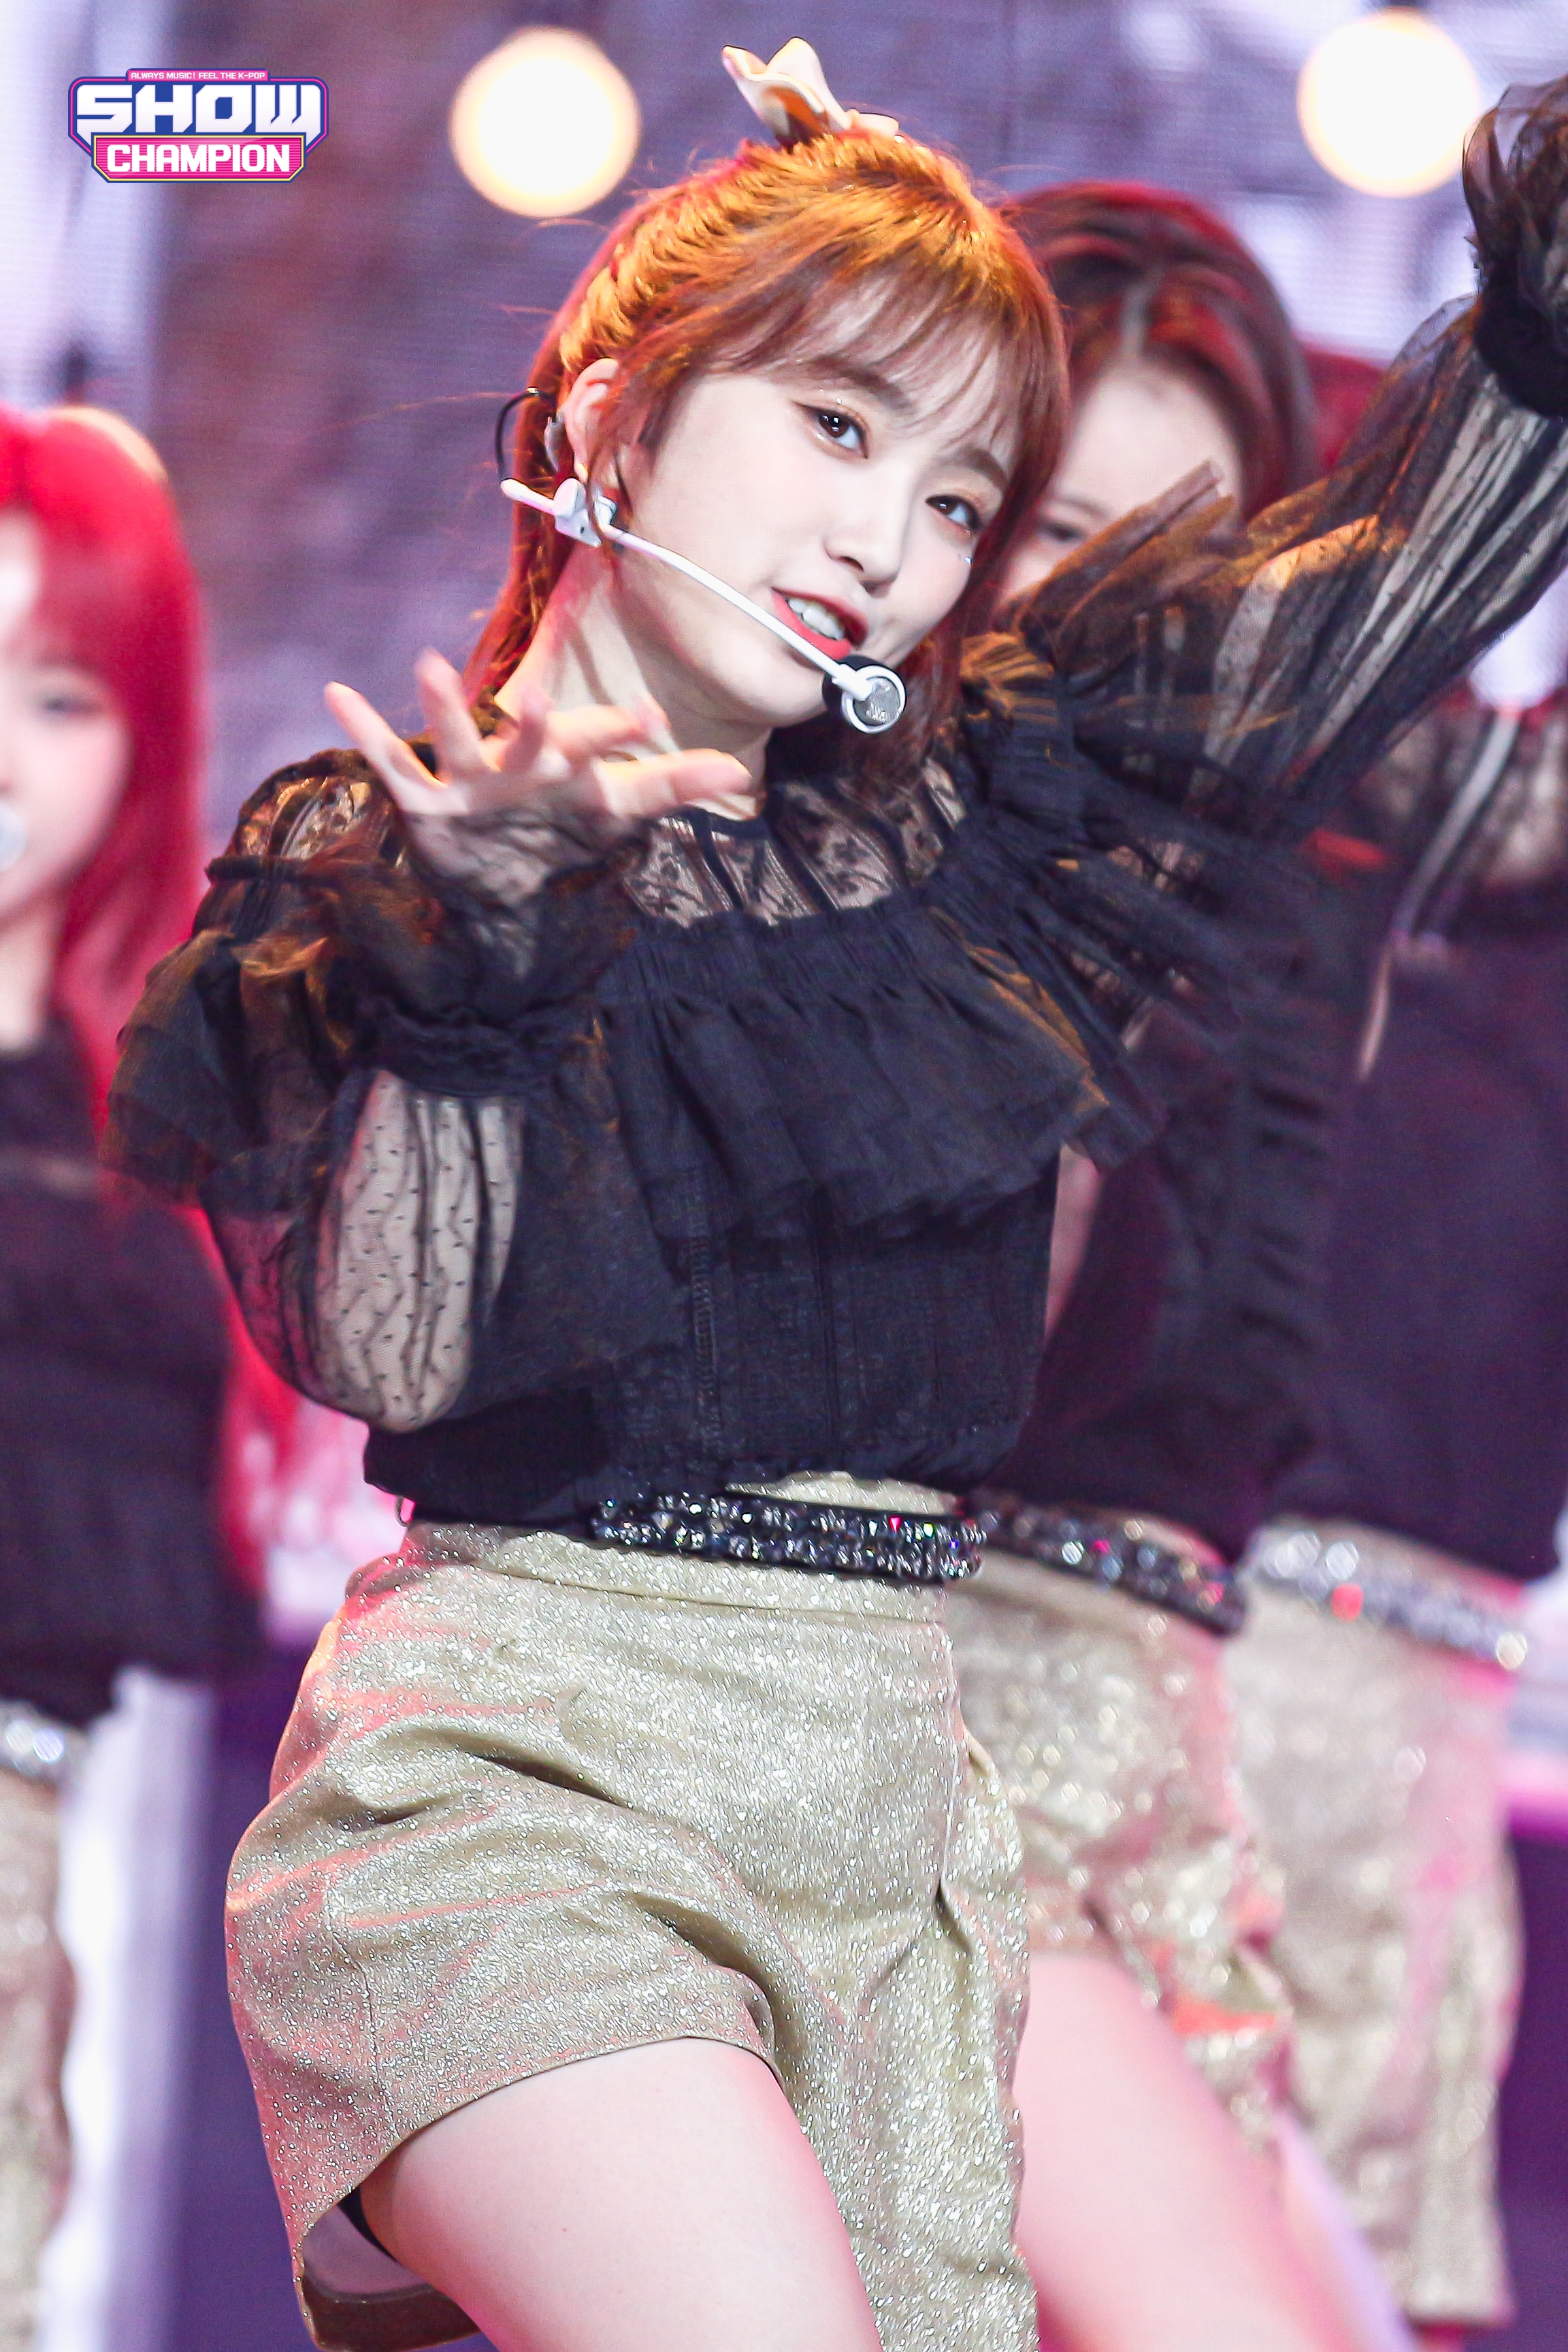
\includegraphics[trim=0 300 0 0, clip, width=.15\textwidth]{images/introduction/nako-unlabelled.jpg}};

        \node[vertex, draw, thick] (faceDetectionModel) at (1, 0) {Face Detection Model};

        \node[inner sep=0pt] (nakoFace) at (6, 3.5) {
            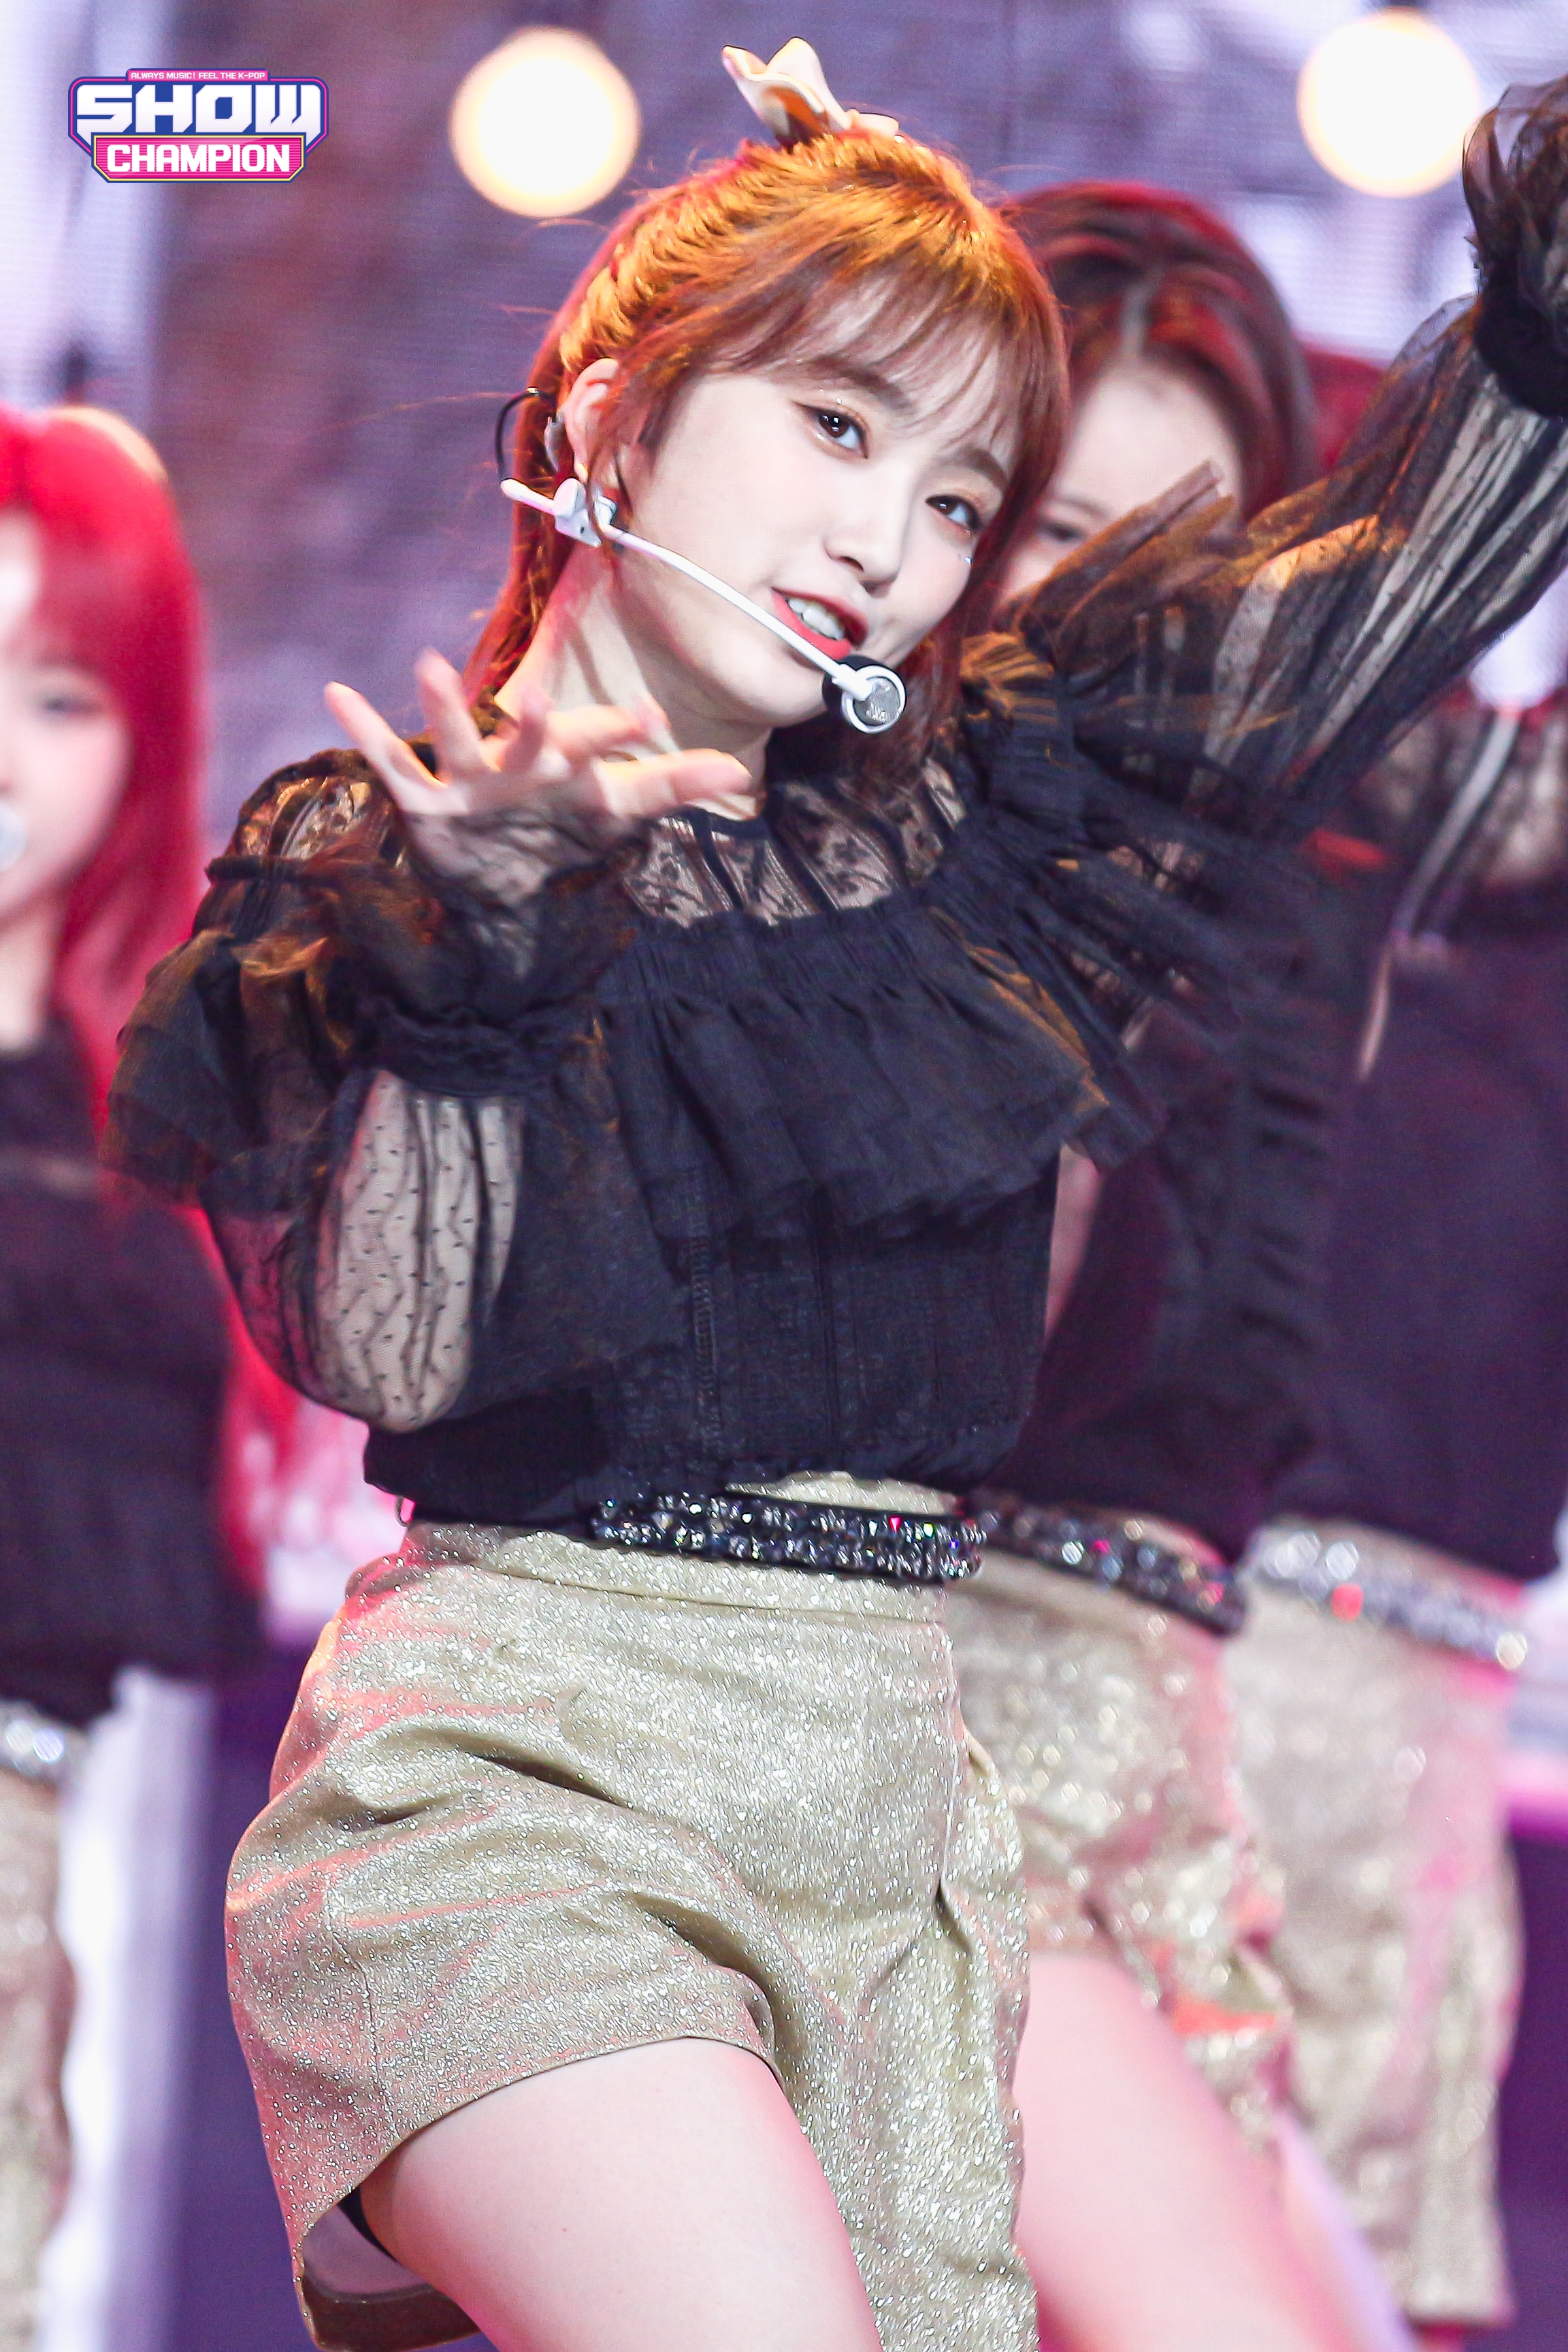
\includegraphics[trim=500 1700 500 80, clip, width=.09\textwidth]{images/introduction/nako-unlabelled.jpg}};
            
        \node[shape=rectangle, font=\small, align=center] (boundingBox) at (6, -4) 
            {$\begin{bmatrix} b_1 \\ \vdots \\ b_k \end{bmatrix}$};

            \node[inner sep=0pt, label={\Large Output image}] (nakoLabelled) at (14.5, 0) {
                \includegraphics[trim=0 75 0 0, clip, width=.23\textwidth]{images/introduction/nako-labelled.png}};

        \draw[edge] (nako) to (faceDetectionModel);
        \draw[edge] (faceDetectionModel) to node[edgeText] {Extract \\ face} (nakoFace);
        \draw[edge] (faceDetectionModel) to node[edgeText] {Get bounding \\ box coordinates} (boundingBox);
        \draw[edge] (nakoFace) to node[edgeText] {Label \\ (using Face Reco- \\ gnition Model)} (nakoLabelled);
        \draw[edge] (boundingBox) to node[edgeText] {Draw red \\ box} (nakoLabelled);
    \end{tikzpicture}
    \caption{IZ*Net Pipeline}
    \label{Figure:Introduction:IZNet-pipeline}
\end{figure}

\footnotetext{Indeed, the face recognition model has trouble with differentiating the JoYuriz trio}

The face detection model is based on the YOLO model \cite{YOLO, YOLOv2, YOLOv3}, while for the face recognition model we experiment with techniques described in the DeepFace \cite{deepface} and FaceNet \cite{facenet} models.
We present the work on the face recognition model first, in \Cref{Section:Face-Recognition} since the initial efforts were spent on that.
The work on the face detection model is presented in \Cref{Section:Face-Detection} and we build the full IZ*Net system in \Cref{Section:Building-the-IZNet-System}.

We will include links to code where applicable, for example one can access the Github repo by clicking \href{https://github.com/nicholaspun/IZ-Net}{\inlinecode{this}}\footnote{I realize this assumes you're on a suitable digital reader, for those that are reading a printed version of this, the repo can be found here: \url{https://github.com/nicholaspun/IZ-Net}}.